\subsection{Системы координат}
\label{sec:coord-systems}

\begin{wrapfigure}{r}{0.27\tw}
	\centering
	\vspace{-1pc}
	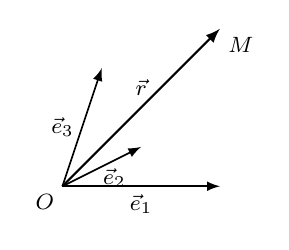
\begin{tikzpicture}[scale=1]
		\footnotesize
		\coordinate (O) at (0, 0);
		\coordinate (E1) at (2, 0);
		\coordinate (E2) at (1, 0.5);
		\coordinate (E3) at (0.5, 1.5);
		\coordinate (M) at (2, 2);
		
		\draw[semithick, -latex] (O) -- (E1);
		\draw[semithick, -latex] (O) -- (E2);
		\draw[semithick, -latex] (O) -- (E3);
		\draw[thick, -latex] (O) -- (M);
		
		\point (O);
		\point (M);
		
		\draw (1, 0) node[anchor=north]{$\vec{e}_1$};
		\draw (0.66, 0.33) node[anchor=north]{$\vec{e}_2$};
		\draw (0.25, 0.75) node[anchor=east]{$\vec{e}_3$};
		\draw (1, 1.05) node[anchor=south]{$\vec{r}$};
		\draw (M) node[anchor=north west]{$M$};
		\draw (O) node[anchor=north east]{$O$};
	\end{tikzpicture}
	\caption{}
	\vspace{-1pc}
	\label{pic:math-coord-sys-decart}
\end{wrapfigure}
Зафиксируем точку $O$ в пространстве и рассмотрим произвольную точку $M$. Вектор $\vec{r} = \overrightarrow{OM}$ называется радиус-вектором точки $M$. Пусть в рассматриваемом пространстве также выбран базис $\{\vec{e}_1, \ldots, \vec{e}_n \}$, тогда совокупность точка $O$ и базиса называется \term{декартовой системой координат}. Причем точка $O$~--- начало координат, а базисные векторы $\vec{e}_1, \ldots, \vec{e}_n$ задают координатные оси.

\begin{wrapfigure}{r}{0.27\tw}
	\centering
	\vspace{-1pc}
	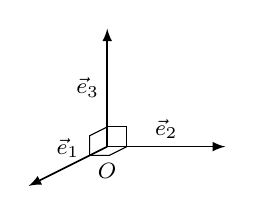
\begin{tikzpicture}[scale=1]
		\footnotesize
		\coordinate (O) at (0, 0);
		\coordinate (E1) at (1.5, 0);
		\coordinate (E2) at (-1, -0.5);
		\coordinate (E3) at (0, 1.5);
%		\coordinate (M) at (2, 2);
		
		\draw[semithick, -latex] (O) -- (E1);
		\draw[semithick, -latex] (O) -- (E2);
		\draw[semithick, -latex] (O) -- (E3);
%		\draw[thick, -latex] (O) -- (M);
		
		\point (O);
%		\point (M);
		
		\draw (-0.5, -0.25) node[anchor=south]{$\vec{e}_1$};
		\draw (0.75, 0) node[anchor=south]{$\vec{e}_2$};
		\draw (0, 0.75) node[anchor=east]{$\vec{e}_3$};
%		\draw (1, 1.05) node[anchor=south]{$\vec{r}$};
%		\draw (M) node[anchor=south]{$M$};
		\draw (0, -0.1) node[anchor=north]{$O$};
		
		\draw (0, 0.25) -- (0.25, 0.25) -- (0.25, 0);
		\draw (0.25, 0) -- (0.027, -0.112) -- (-0.223, -0.112);
		\draw (0, 0.25) -- (-0.223, 0.138) -- (-0.223, -0.112);
	\end{tikzpicture}
	\caption{}
	\vspace{-1pc}
	\label{pic:math-coord-sys-ord-basis}
\end{wrapfigure}
Однако пользоваться представлением векторов в произвольном базисе довольно сложно, поэтому рассмотрим специальный тип~--- \term{орто\-нор\-ми\-рованный базис}~--- это такой базис, базисные векторы которого попарно ортогональны, и длина каждого равна единице.

\term{Прямоугольной декартовой системой координат} (ПДСК) называют декартову систему координат с ортонормированным базисом. В практических задачах использовать ПДСК не всегда удобно, поэтому также рассмотрим другие системы координат. 

\begin{wrapfigure}{r}{0.27\tw}
	\centering
	\vspace{-1pc}
	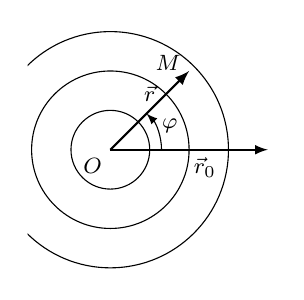
\begin{tikzpicture}[scale=1]
		\clip(-1.05, -1.55) rectangle (2.1, 1.55);
	
		\footnotesize
		\coordinate (O) at (0, 0);
		\coordinate (E1) at (2, 0);
%		\coordinate (E2) at (1, 0.5);
%		\coordinate (E3) at (0.5, 1.5);
		\coordinate (M) at (1, 1);
		
		\draw[semithick, -latex] (O) -- (E1);
%		\draw[semithick, -latex] (O) -- (E2);
%		\draw[semithick, -latex] (O) -- (E3);
		\draw[thick, -latex] (O) -- (M);
		\draw[-latex] (0.65, 0) arc(0:45:0.65);
		
		\foreach \r in {0.5, 1, 1.5} {
			\draw (O) circle(\r);
		};
		
		\point (O);
		\point (M);
		
		\draw (1.2, 0) node[anchor=north]{$\vec{r}_0$};
%		\draw (0.66, 0.33) node[anchor=north]{$\vec{e}_2$};
%		\draw (0.25, 0.75) node[anchor=east]{$\vec{e}_3$};
		\draw (0.5, 0.5) node[anchor=south]{$\vec{r}$};
		\draw (0.55, 0.3) node[anchor=west]{$\varphi$};
		\draw (1, 0.9) node[anchor=south east]{$M$};
		\draw (O) node[anchor=north east]{$O$};
	\end{tikzpicture}
	\caption{}
	\label{pic:math-coord-sys-polar}
\end{wrapfigure}
На плоскости, то есть в пространстве $\R^2$, имеющем размерность два, часто применяется \term{полярная система координат}. В ней координатами вектора является его длина $r$~--- расстояние до точки от начала отсчёта, и угол $\varphi$ радиус-вектора с начальной ось.

Пусть $(x,y)$~--- координаты некоторого вектора в ПДСК на $\R^2$, тогда не сложно получить, что его координаты в полярной системе координат (начальная ось совпадает с осью $Ox$)  удовлетворяют следующим соотношениям:
\begin{equation}
	\begin{cases}
		r = \sqrt{x^2 + y^2},\\
		\sin \varphi = y/r,\\
		\cos \varphi = x/r.
	\end{cases}
	\quad \Leftrightarrow \quad
	\begin{cases}
		x = r \cos \varphi,\\
		y = r \sin \varphi.
	\end{cases}
\end{equation}

\begin{wrapfigure}{r}{0.35\tw}
	\centering
%	\vspace{-1pc}
	\begin{tikzpicture}[scale=1]
		\clip(-1.3, -1.1) rectangle (2.5, 2.5);
	
		\footnotesize
		\coordinate (O) at (0, 0);
		\coordinate (E1) at (2.3, 0);
		\coordinate (E2) at (0, 2.3);
		\coordinate (E3) at (-1, -1);
		\coordinate (M) at (0.8, 1.3);
		\coordinate (M') at (0.8, -0.48);
		\coordinate (M'') at (1, -0.6);
		
		\draw[semithick, -latex] (O) -- (E1);
		\draw[semithick, -latex] (O) -- (E2);
		\draw[semithick, -latex] (O) -- (E3);
		\draw[thick, -latex] (O) -- (M);
		
		\draw [dashes] (0, 1.78) -- (M) -- (M');
		\draw [dashes] (M'') -- (O);
		\draw [dashes] (1.28, 0) -- (M') -- (-0.48, -0.48);
		
		\draw (O) ellipse(2 and 0.7);
		\draw (0, 1.78) ellipse(2 and 0.7);
		
		\draw [-latex](-0.2, -0.2) arc(-99.4:-75.76:1.22);

        \foreach \p in {O, M, M', M''} {
            \point (\p);
        };
		
		\draw (0.5, 0.65) node[anchor=south east]{$\vec{r}$};		
		\draw (0.05, -0.15) node[anchor=north]{$\varphi$};
		\draw (0.42, -0.2) node[anchor=west]{$r$};
		\draw (0.8, 0.4) node[anchor=west]{$h$};
		\draw (M) node[anchor=south west]{$M$};
		\draw (O) node[anchor=south east]{$O$};
		
		\draw (E1) node[anchor=north]{$y$};
		\draw (E2) node[anchor=east]{$z$};
		\draw (E3) node[anchor=east]{$x$};
	\end{tikzpicture}
	\caption{}
	\label{pic:math-coord-sys-cyl}
	\vspace{-2pc}
\end{wrapfigure}
Теперь пусть $(x, y, z)$~--- координаты некоторого вектора в ПДСК на~$\R^3$. Обозначим за $h$~--- длину проекции этого вектора на ось $z$, $r$~--- длину его проекции на плоскость $Oxy$, $\varphi$~--- угол между проекцией на плоскость $Oxy$ и осью $Ox$. Тогда тройка $(r, \varphi, h)$~--- координаты рассматриваемого векторы в \term{цилиндрической системе координат}, и верно представление
\begin{equation}
	\begin{cases}
		r = \sqrt{x^2 + y^2},\\
		\sin \varphi = y/r,\\
		\cos \varphi = x/r,\\
		h = z.
	\end{cases}
	\quad \Leftrightarrow \quad
	\begin{cases}
		x = r \cos \varphi,\\
		y = r \sin \varphi,\\
		z = h.
	\end{cases}
\end{equation}

\begin{wrapfigure}{r}{0.35\tw}
	\centering
	\vspace{-2.5pc}
	\begin{tikzpicture}[scale=1]
		\clip(-1.3, -1.1) rectangle (2.5, 2.5);
%	
%		\foreach \x in {-5, -4.9,...,5} {
%			\draw [line width=.1pt] (\x, -5) -- (\x, 5);
%		};
%		
%		\foreach \x in {-5, -4,..., 5} {
%			\draw [line width=.4pt] (\x , -5) -- (\x , 5);
%		};
%		
%		\foreach \y in {-5, -4,..., 5} {
%			\draw [line width=.4pt] (-5, \y) -- (5, \y);
%		};
%		
%		\foreach \y in {-5, -4.9,..., 5} {
%			\draw [line width=.1pt] (-5, \y) -- (5, \y);
%		};
	
		\footnotesize
		\coordinate (O) at (0, 0);
		\coordinate (E1) at (2.3, 0);
		\coordinate (E2) at (0, 2.3);
		\coordinate (E3) at (-1, -1);
		\coordinate (M) at (0.8, 1.3);
		\coordinate (M') at (0.8, -0.48);
		\coordinate (M'') at (1, -0.6);
		
		\draw[semithick, -latex] (O) -- (E1);
		\draw[semithick, -latex] (O) -- (E2);
		\draw[semithick, -latex] (O) -- (E3);
		\draw[thick, -latex] (O) -- (M);
		
		\draw [dashes] (0, 1.78) -- (M) -- (M');
		\draw [dashes] (M'') -- (O);
		\draw [dashes] (0, 2) arc(90:-90:1.05 and 2);
		\draw [dashes] (M') -- (-0.48, -0.48);
		\draw [dashes] (M') -- (1.28, 0);
%		\draw[-latex] (1.02, 0) arc(0:45:1 and 0.4);
		
		\draw (O) circle(2);
		\draw (0, 2) arc(90:270:0.7 and 2);
		\draw (2, 0) arc(360:180:2 and 0.7);
		
		\draw [-latex](-0.2, -0.2) arc(-99.4:-75.76:1.22);
		\draw [-latex](0.29, -0.18) arc(-9.44:18:1.22); 
%		\draw (O) ellipse(0.6 and 0.21);
%		\draw (-1, 0) circle(1.3);
		
		
		\foreach \p in {O, M, M', M''} {
            \point (\p);
        };
	
		
		\draw (0.5, 0.6) node[anchor=south east]{$\vec{r}$};		
%		\draw (1.05, -0.25) node[anchor=west]{$x$};
%		\draw (0.2, -0.45) node[anchor=north]{$y$};
%		\draw (0.75, 0.3) node[anchor=west]{$z$};
		\draw (0.3, 0.15) node[anchor=west]{$\varphi$};
		\draw (0.05, -0.15) node[anchor=north]{$\theta$};
		\draw (M) node[anchor=west]{$M$};
		\draw (O) node[anchor=south east]{$O$};
		
		\draw (E1) node[anchor=north]{$y$};
		\draw (E2) node[anchor=east]{$z$};
		\draw (E3) node[anchor=east]{$x$};
	\end{tikzpicture}
	\caption{}
	\label{pic:math-coord-sys-sphere}
	\vspace{-1.5pc}
\end{wrapfigure}
Остается рассмотреть \term{сферическую систему координат}. Здесь координатами точки будет длина $r$ радиус-вектора $\vec{r}$ и два угла: $\theta$~--- угол между радиус-вектором и плоскостью $Oxy$ и $\varphi$~--- угол между проекцией радиус-вектора на плоскость $Oxy$ и осью $Ox$. Верны формулы перехода:
\begin{equation}
	\begin{cases}
		r = \sqrt{x^2 + y^2 + z^2},\\
		\theta = \arcsin{z/r},\\
		\sin \varphi = y/r,\\
		\cos \varphi = x/r.
	\end{cases}
	\quad \Leftrightarrow \quad
	\begin{cases}
		x = r \cos \theta \cos \varphi	,\\
		y = r \cos \theta \sin \varphi,\\
		z = r \sin \theta.
	\end{cases}
\end{equation}
